\documentclass[../portafolio.tex]{subfiles}



\begin{document}

\section{Interpolación} 

\hfill \textbf{Fecha de la actividad:} 28 de octubre de 2022

\medskip


%-----------------------------------------------------%
%-----------------------------------------------------%
%-----------------------------------------------------%

\subsection{Objetivo de la clase}

La interpolación es la obtención de nuevos puntos partiendo del conocimiento de un conjunto de puntos \cite{interpol}. El objetivo de este laboratorio fue aprender a hacer interpolaciones polinomiales con 3 métodos distintos: construyendo polinomios de Lagrange, usando la interpolación \textit{spline} cúbica y usando la inversa de la matriz de Vandermonde. Para ello, se trabajó con datos de la cantidad de manchas solares por año.

\vspace{2mm}
En este laboratorio trabajé junto a Eduardo Escudero y Mauricio Bastías.



%-----------------------------------------------------%
%-----------------------------------------------------%
%-----------------------------------------------------%

\subsection{Desarrollo del laboratorio}

Se comenzó trabajando usando la inversión de la matriz de Vandermonde, para ello en la línea 9 y 10 del código \ref{C1-interp} se creó la matriz y en la línea 12 se resolvió el sistema $M\times a = B$, donde M es la matriz de Vandermonde y B es \texttt{Manchas2} obteniéndose de esta forma \texttt{a}. Luego, en la línea 14 se creó una función que representaba el polinomio que graficaba la curva de la interpolación. Finalmente, se introdujo todo esto en un ciclo \texttt{for} para interpolar todos los datos en intervalos de 5 puntos, pues este método daba error cuando se intentaba interpolar con más de cinco nodos. El número 51 que aparece en la línea 1 del código hacer referencia a que se hicieron 51 interpolaciones que estaban unidas entre sí por un nodo.De este modo se obtuvo el gráfico \ref{vanderm}.

\begin{listing}[h]
    \begin{minted}[
frame=lines,
framesep=2mm,
baselinestretch=1.2,
bgcolor=LightGray,
fontsize=\footnotesize,
linenos
]
{python}
for m in range(51):
    año2 = año[m*4:5+m*4]
    manchas2 = manchas[m*4:5+m*4]

    dim = año2.size

    vandermonde = np.ones( [dim,dim] )

    for i in range(1,dim):
        vandermonde[:,i]= año2**i

    a = Resolver(vandermonde, manchas2)

    def p(x,a):
        pol=0.0
        for n in range(len(a)):
            pol= pol + a[n] * x**n
        return pol
    \end{minted}
\caption{Fragmento de código en el cual se interpolaron los datos usando la inversión de la matriz de Vandermonde.}
\label{C1-interp}
\end{listing}



El segundo método utilizado fue el de los polinomios de Lagrange. En este caso, al igual que en el anterior, se tuvo que interpolar por intervalos de 5 nodos, para ello se escribió el código \ref{C2-interp} donde se creó una función dentro de una iteración en la línea 7 que construía los polinomios de Lagrange. De este modo, se creó el gráfico \ref{lagr1}.
 
\begin{listing}[]
    \begin{minted}[
frame=lines,
framesep=2mm,
baselinestretch=1.2,
bgcolor=LightGray,
fontsize=\footnotesize,
linenos
]
{python}
for m in range(51):
    año2 = año[m*4:5+m*4]
    manchas2 = manchas[m*4:5+m*4]

    N= len(año2)

    def f(x):
        pol = 0.0
        for i in range(N):
            Li = manchas2[i]
            for j in range(N):
                if j != i:
                    Li = Li * (x-año2[j]) / (año2[i] - año2[j])
            pol= pol + Li
        return(pol)
    \end{minted}
\caption{Fragmento de código utilizado para construir los polinomios de Lagrange y posteriormente crear el gráfico \ref{lagr1} con los polinomios obtenidos. }
\label{C2-interp}
\end{listing}



\begin{figure}[H]
    \centering
    \begin{subfigure}[b]{0.49\textwidth}
        \centering
        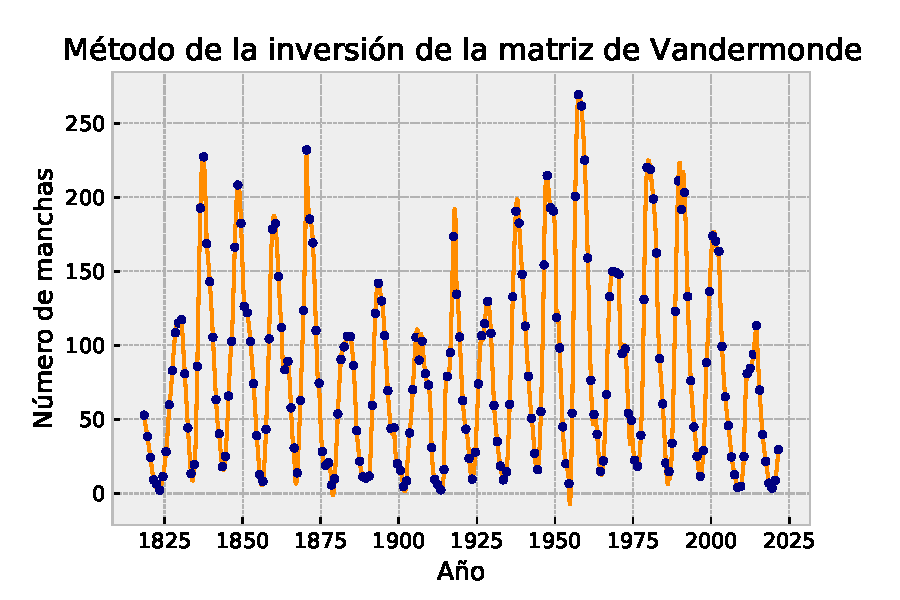
\includegraphics[width=\textwidth]{tex/img/vandermonde.pdf}
        \caption{}
        \label{vanderm}
    \end{subfigure}
    \hfill
    \begin{subfigure}[b]{0.49\textwidth}
        \centering
        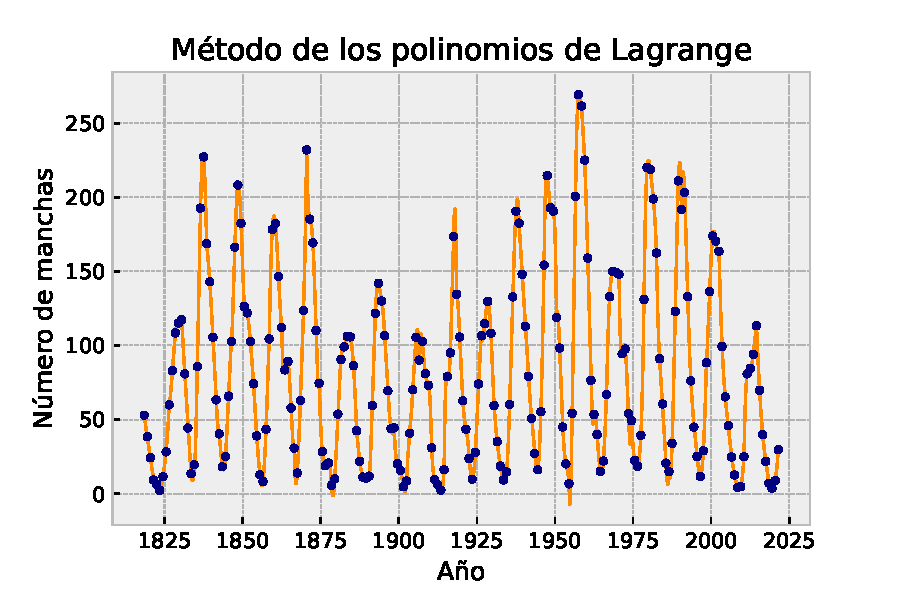
\includegraphics[width=\textwidth]{tex/img/lagrange1.pdf}
        \caption{}
        \label{lagr1}
    \end{subfigure}
    \hfill
    \begin{subfigure}[b]{0.49\textwidth}
         \centering
         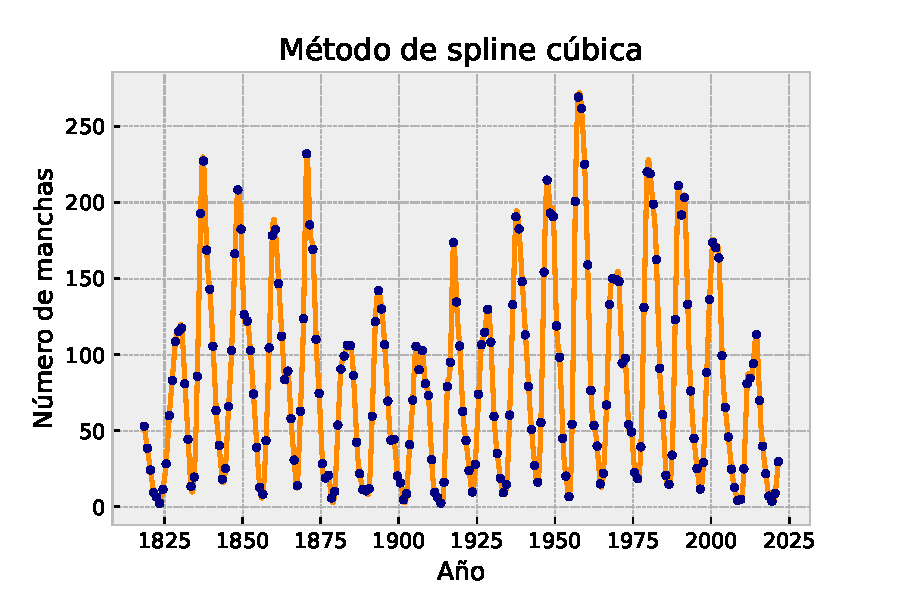
\includegraphics[width=\textwidth]{tex/img/sp.pdf}
         \caption{}
         \label{sp}
     \end{subfigure}
    \caption{Gráficos del promedio de número de manchas solares con respecto al año, donde los punto azules representan los datos y la curva naranja se obtuvo al interpolar con los métodos que aparecen en sus respectivos títulos.}
    \label{--}
\end{figure}


Para el último caso, se interpoló utilizando splines cúbica. Este método es un conjunto de polinomios de tercer grado que se genera a partir de un conjunto de puntos \cite{spline}. Al utilizar este método, a diferencia de la matriz de Vandermonde y los polinomio de Lagrange, no se tuvieron que interpolar los datos utilizando intervalos, pues bastó con interpolar todos los datos en un solo intervalo. 

\vspace{2mm}
Para interpolar usando spline cúbica se creó el código \ref{C3-interp}. Con ayuda de la función cspline del programa \textit{spline} se creó en la primera línea la función \texttt{csp} que creó una función que interpolaba todos los puntos, luego para graficar la curva en la línea 2 y 3 se evaluó con la función \texttt{csp} 10000 valores ubicados en el intervalo $\left[1818,2021 \right[$. La función cspline interpola utilizando polinomio cúbicos y retorna una función que pasa por todos los nodos, de este modo se obtuvo el gráfico \ref{sp}.


\begin{listing}[]
    \begin{minted}[
frame=lines,
framesep=2mm,
baselinestretch=1.2,
bgcolor=LightGray,
fontsize=\footnotesize,
linenos
]
{python}
csp = sp.cspline(año, manchas)
x = np.linspace( np.min(año), np.max(año), 10000, endpoint=False)
plt.plot(x, csp(x))
    \end{minted}
\caption{Código utilizado para interpolar usando spline cúbico.}
\label{C3-interp}
\end{listing}

\vspace{2mm}
Finalmente, al comparar los gráficos \ref{vanderm} y \ref{lagr1} se puede observar en ambos casos que al hacer un acercamiento se obtiene el gráfico de la figura \ref{acerc} donde se aprecia que la curva no es suave, esto se debe a que al interpolar se tuvo que separar en 51 intervalos, quedando de este modo 51 interpolaciones donde en las conexiones de dichas interpolaciones quedaron puntas. Por otro lado, al usar el método spline cúbica la curva quedó suave en todas sus partes.

\begin{figure}
    \centering
    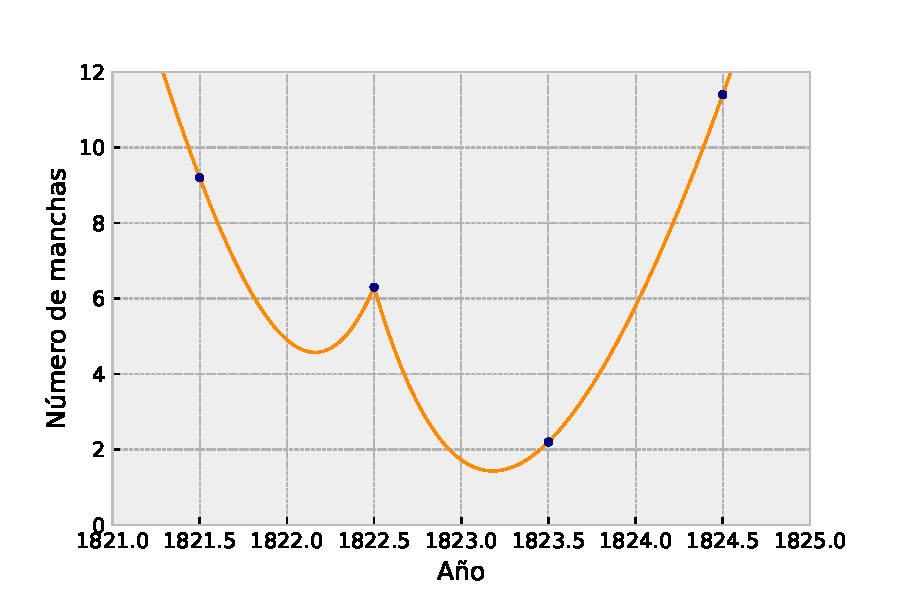
\includegraphics{tex/img/acercamiento.pdf}
    \caption{Acercamiento del gráfico \ref{vanderm} y \ref{lagr1}}
    \label{acerc}
\end{figure}

%-----------------------------------------------------%
%-----------------------------------------------------%
%-----------------------------------------------------%

\subsection{Conclusión}

En este laboratorio se trabajó con datos que entregaban la información del promedio de las manchas solares desde el año 1818 hasta el 2021. Estos datos se interpolaron con 3 métodos distintos obteniéndose los gráficos \ref{vanderm}, \ref{lagr1} y \ref{sp} que corresponden a la curva obtenida al interpolar con los métodos de la matriz de Vandermonde, polinomio de Lagrange y spline cúbica, respectivamente. Analizando y comparando los tres gráficos se pudo concluir que al utilizar el método de spline cúbica  se pueden obtener resultados más útiles, al menos en este caso, para predecir que sucede entre los nodos, pues al utilizar los polinomios de Lagrange y la inversa de la matriz de Vandermonde se obtienen curvas que no son suaves en todas sus partes y por ende no estimará tan bien el comportamiento de los datos como cuando se usa spline cúbica.

\vspace{2mm}
En esta actividad aprendí que cuando se tienen ciertos datos en los que se presentan variables independientes y variables dependientes, se puede intentar estimar el comportamiento entre dos nodos (datos). Siendo esto muy útil para predecir ciertos acontecimientos en diversas áreas, tales como la economía, la sociología, etc.

\vspace{2mm}
En el desarrollo de esta actividad me hubiera gustado que se explicara un poco más el método de interpolación \textit{spline} cúbica, ya que al leer el código de esta función no entendí casi nada y solo aprendí a utilizarla copiando la función, por lo que no supe como explicar el desarrollo cuando utilicé este método.



\end{document}